\documentclass[11pt, oneside]{article}   	% use "amsart" instead of "article" for AMSLaTeX format
\usepackage{geometry}                		% See geometry.pdf to learn the layout options. There are lots.
\geometry{letterpaper}                   		% ... or a4paper or a5paper or ... 
%\geometry{landscape}                		% Activate for for rotated page geometry
%\usepackage[parfill]{parskip}    		% Activate to begin paragraphs with an empty line rather than an indent
\usepackage{graphicx}				% Use pdf, png, jpg, or eps� with pdflatex; use eps in DVI mode
								% TeX will automatically convert eps --> pdf in pdflatex		
\usepackage{amssymb}
\usepackage{amsmath}

\title{More sums}
%\author{The Author}
\date{}							% Activate to display a given date or no date

\graphicspath{{/Users/telliott_admin/Dropbox/Tex/png/}}

\begin{document}
 
\maketitle
%\section{}
% \subsection*{R code}
% \begin{lstlisting}  \end{lstlisting}
% \begin{center} 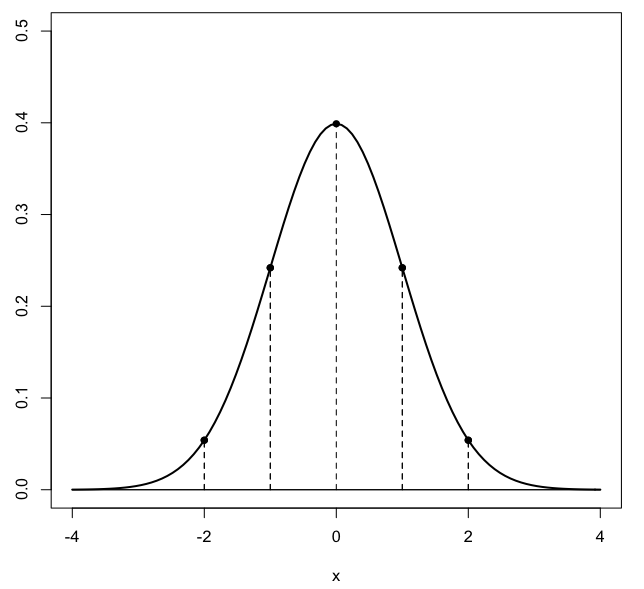
\includegraphics [scale=0.4] {gauss3.png} \end{center}
% \begin{bmatrix} a  &  b \\ c  &  d \end{bmatrix}
% \bigg |_

\large
We have shown in other write-ups, and you can easily verify by searching that the sum of the integers between $1$ and $n$ is 
\[ 1 + 2 + \dots + n = \sum\limits_{k=1}^n k = \frac{n(n+1)}{2} \]
The next one, the sum of the squares of the first $n$ integers, is useful for certain derivations in calculus (e.g. the Riemann sum to integrate $y=x^2$)
\[ 1^2 + 2^2 + \dots + n^2 = \sum\limits_{k=1}^n k^2 = \frac{n(n+1)(2n+1)}{6} \]
I was quite surprised to find that the sum of cubes is also simple and frankly, amazing
\[ 1^3 + 2^3 + \dots + n^3 = \sum\limits_{k=1}^n k^3 = \frac{n^2(n+1)^2}{2^2} = [\ \frac{n(n+1)}{2}\ ]^2 = [\ \sum\limits_{k=1}^n k \ ] ^2 \]
\begin{equation}
\boxed{ \sum\limits_{k=1}^n k^3 = [\ \sum\limits_{k=1}^n k \ ] ^2}
\end{equation}
Let's just try to prove the last formula using induction.

The "base case" is pretty simple.  For $n=2$
\[ 1^3 + 2^3 = 1 + 8 = 9 \]
and
\[ \frac{n^2(n+1)^2}{2^2} = \frac{2^2(3^2)}{2^2} = 3^2 = 9 \]
Check.  Now for the induction step what we need to show is that what we get assuming the formula for $n$ is correct and then adding the term $(n+1)^3$
\begin{equation}
\boxed{ \frac{n^2(n+1)^2}{2^2} + (n+1)^3}
\end{equation}
is equal to what we get by plugging $n+1$ into the formula.
\begin{equation}
\boxed{ \frac{(n+1)^2(n+2)^2}{2^2}}
\end{equation}
We need to show that eqn 2 is equal to eqn 3.  
\[ \frac{n^2(n+1)^2}{2^2} + (n+1)^3 = \frac{(n+1)^2(n+2)^2}{2^2} \]
First, we can factor out and cancel $(n+1)^2$ from both sides.  So then we have
\[ \frac{n^2}{2^2} + (n+1) \stackrel{?}{=} \frac{(n+2)^2}{2^2} \]
\[ n^2 + 4(n+1) \stackrel{?}{=} (n+2)^2 \]
Sure, that looks correct!  And we're done with the proof by induction, so we can put a little box.

\noindent
$\blacksquare$

\subsection*{Looking deeper}

\[ \sum\limits_{k=1}^n k^3 = [\ \sum\limits_{k=1}^n k \ ] ^2 \]

I wanted to try to understand something more about why this is true.  A simple web search revealed the answer.  Here's an interesting pattern for the cubes of integers that I'd never seen before

\[ 1^3 = 1 \]
\[ 2^3 = 8 = 3 + 5 \]
\[ 3^3 = 27 = 7 + 9 + 11 \]
\[ 4^3 = 64 = 13 + 15 + 17 + 19 \]
\[ 5^3 = 125 = 21 + 23 + 25 + 27 + 29  \]

If you want a formula for $n^3$, notice that the first term is $n^2 - n + 1$ and the last term is $n^2 - n + 2n - 1$, and the number of terms for each sum equals $n$.  (There are $n$ odd numbers between $1$ and $2n-1$).

In other words, the sum of all the cubes of integers from $1^3$ to $n^3$ is equal to the sum of all the odd numbers up to $n^2 - n + 2n - 1 = n^2 + n - 1$.

How many of these numbers are there?  A little thought should convince you that the correct answer is $(n^2 + n)/2$.  For example, with $n=5$, our last odd number is $5^2 + 5 - 1 = 29$, and we have $(25 + 5)/2 = 15$ terms.

We want the sum of the first $(n^2 + n)/2$ odd numbers.

Let's look at another pattern
\[ 1 = 1 \]
\[ 2^2 = 4 = 1 + 3 \]
\[ 3^2 = 9 = 1 + 3 + 5 \]
\[ 4^2 = 16 = 1 + 3 + 5 + 7 \]
\[ 5^2 = 25 = 1 + 3 + 5 + 7 + 9 \]

The \emph{odd number theorem} says that the sum of the first $n$ odd numbers is equal to $n^2$.  We want the sum of the first $(n^2 + n)/2$ odd numbers, so that's $((n^2 + n)/2)^2$.  And that's how we get our formula.

\end{document}  